% !TEX root = Thesis.tex
\chapter{Introduction}\label{sec:Intro}

  In the late nanoscale CMOS era, automated layout generation of advanced technologies has drawn more attention due to the growing demand in industry. As the complexity of the advanced nodes for analog circuit increases, the layout constraints and the expanding performance requirements become major productivity bottlenecks. Lately, in order to alleviate the impact from process variation beyond the transistor level as well as striving for excellent performance, analog layout design mostly relies on designers' expertise. However, the iterative refinement on manual design damages the productivity of analog layout. Therefore, it is more efficient to enroll the know-how from existing designs instead of generating a new one. To migrate layout template via preservation becomes a plus.

  For analog layout, reusability relies on the similarity such that part of source layout can be reused to add new modules or layers on target layout with minor modification. To preserve the design knowledge from the template layouts, the devices' relative positions and the routing behaviors should be considered thoroughly. Typical analog constraints such as symmetry and proximity constraints fundamentally regulate the placement. On the other hand, wire symmetry and topological matching are critical to analog routing. Placement and routing extracted from the template layout can benefit layout migration. In other words, more informations are extracted from template layout, more circuit characteristics are preserved. Currently, analog layout preservation pays more attention on placement~\cite{cart-hammouda-dac06,cbc-bhattacharya-dac04,Wang_ALRGP_TODAES2011} 
  for topology extraction. However, seldom do we study routing behavior extraction in previous works. In all, a solution to preserve the correlation during layout retargeting, or so-called layout migration is critical.


  \begin{figure}
    \centering
    \begin{subfigure}[t]{4cm}
    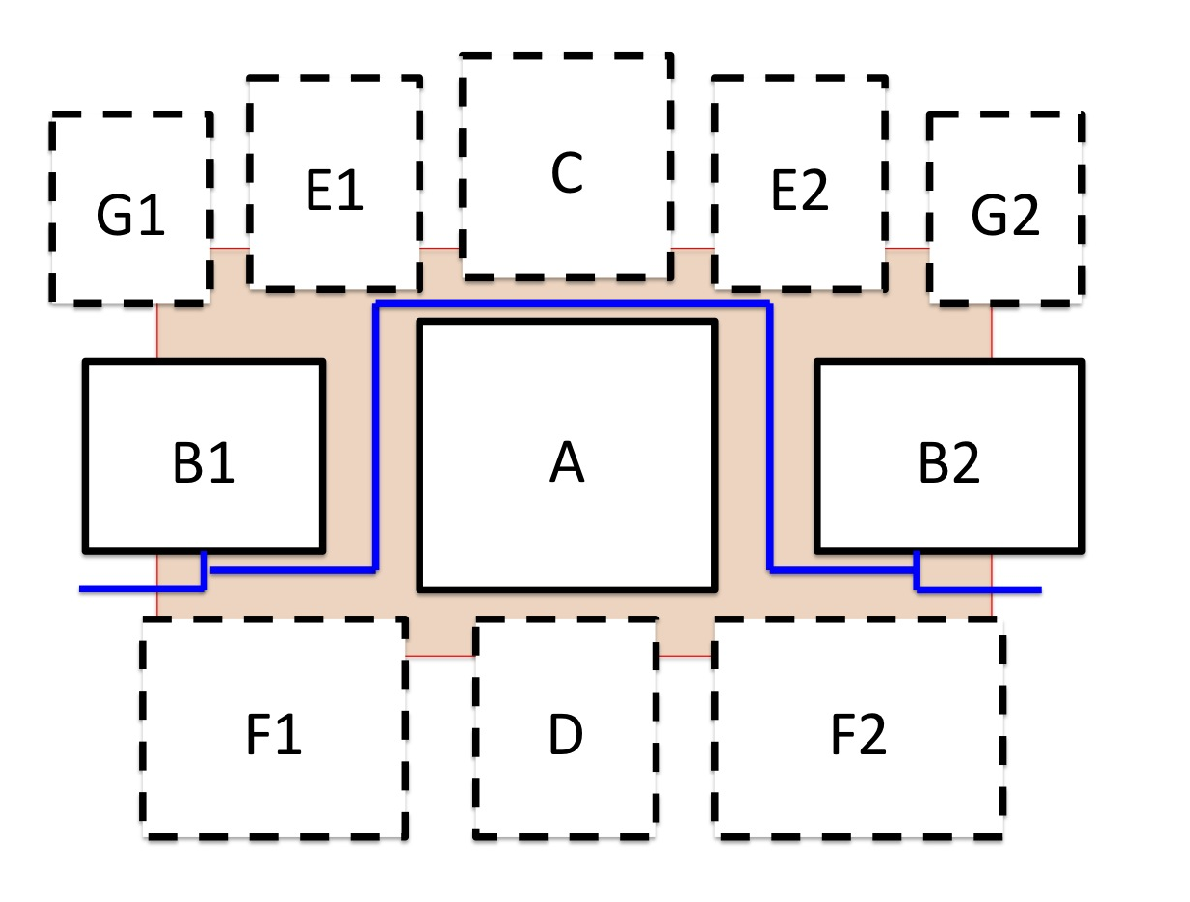
\includegraphics[width=4cm]{Fig/RoutingPreserv_a.eps}
    \caption{Reference template layout}
    \label{fig:RoutingPreserv_A}
    \end{subfigure}
    \begin{subfigure}[t]{4cm}
    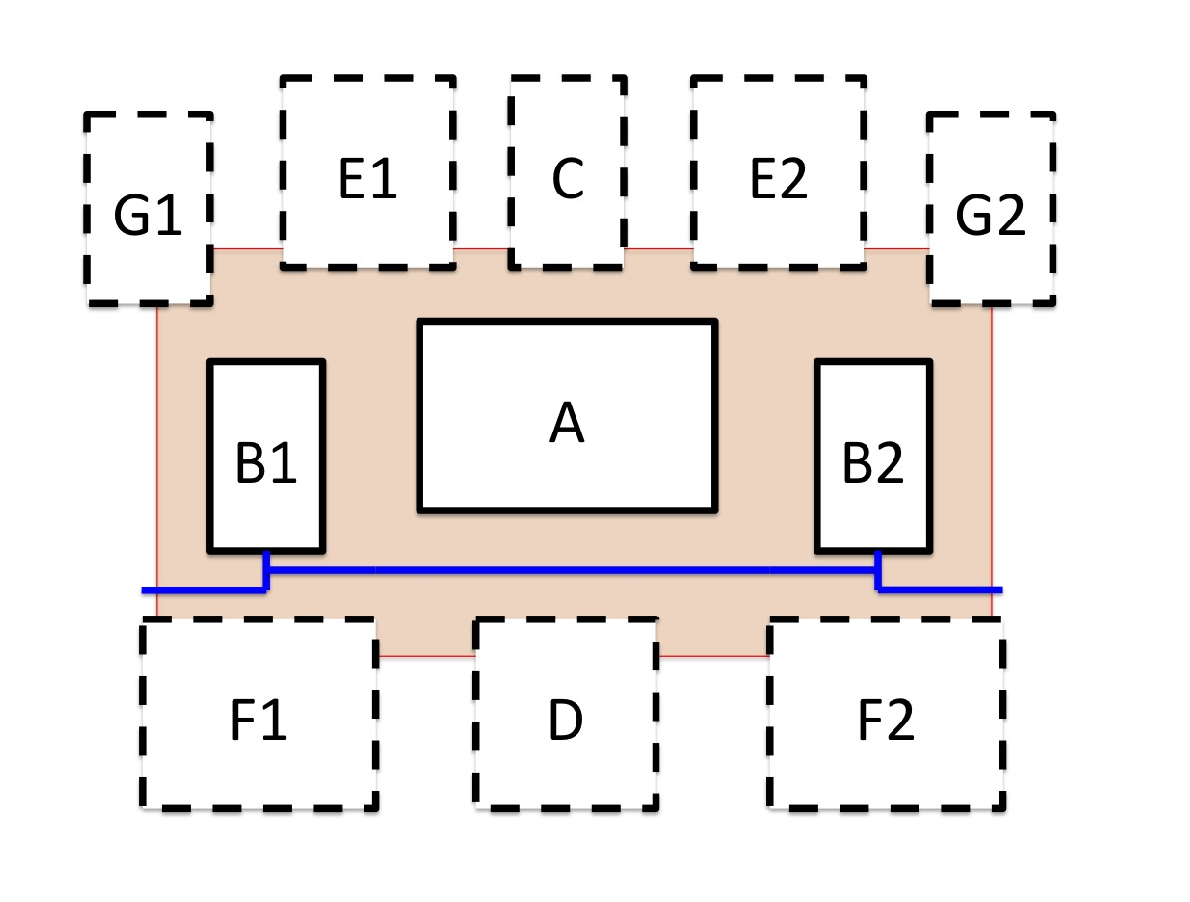
\includegraphics[width=4cm]{Fig/RoutingPreserv_b.eps}
    \caption{Non-preserved automatic routing}
    \label{fig:RoutingPreserv_B}
    \end{subfigure}
    %}
    \begin{subfigure}[t]{4cm}
    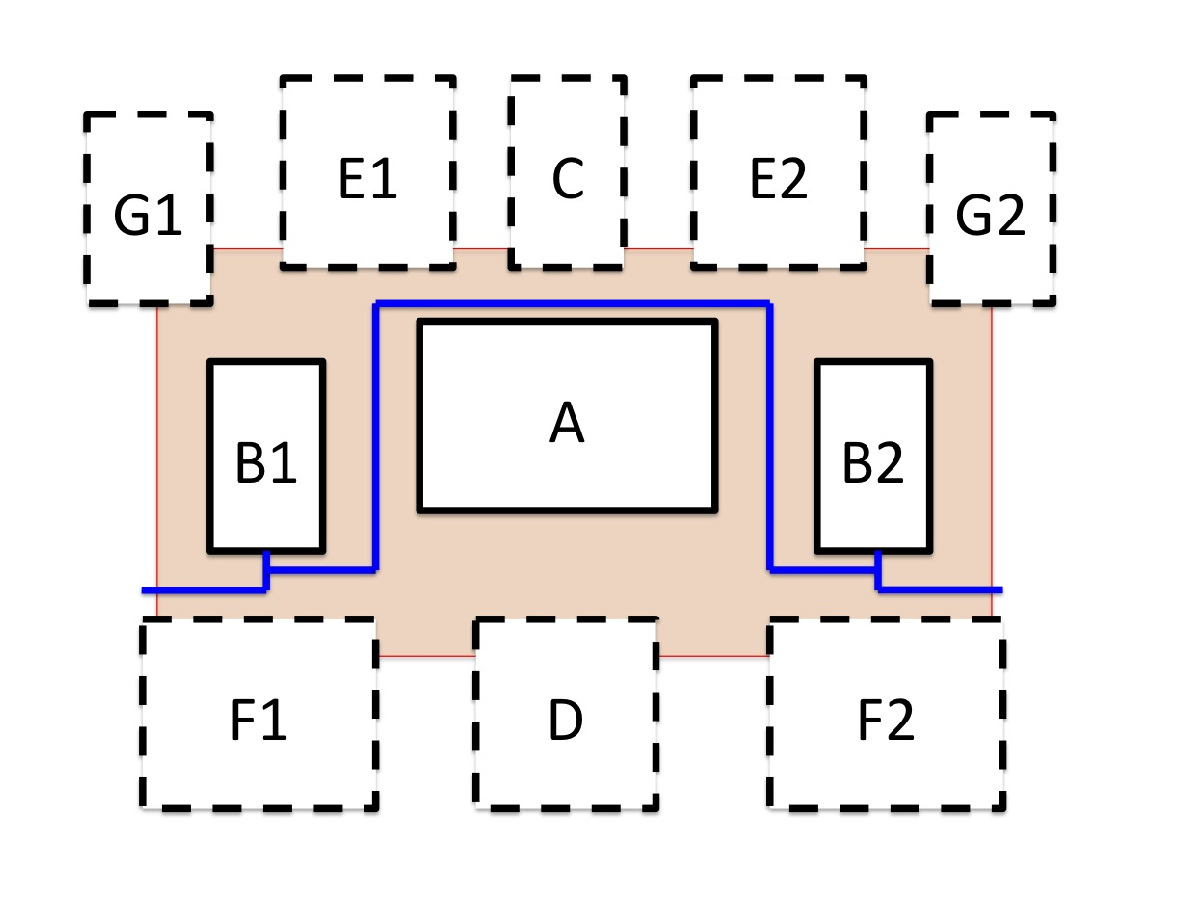
\includegraphics[width=4cm]{Fig/RoutingPreserv_c.eps}
    \caption{Preserved routing}
    \label{fig:RoutingPreserv_C}
    \end{subfigure}
    %}
    
    %\subfigure[Timing and simulation results]{
    %\label{fig:RoutingPreserv_d}
    %\epsfig{file=Fig/Prototyping_d.eps,width=4cm}
    %}
    \caption{Analog layout generation with different configuration. (a) Reference layout with complete placement and routing. (b) non-preserved automatic routing considering usual constraints only. (c) layout generation considering preserved routing characteristics. (d) simulation results in umc65nm technology.}
    \label{fig:RoutingPreserv}
  \end{figure}